% !TEX program = xelatex

\documentclass{resume}
\usepackage{graphicx}
\usepackage{tabu}
\usepackage{multirow}
\usepackage{zh_CN-Adobefonts_external} % 
%\usepackage{zh_CN-Adobefonts_external} % Simplified Chinese Support using external fonts (./fonts/zh_CN-Adobe/)
%\usepackage{zh_CN-Adobefonts_internal} % Simplified Chinese Support using system fonts

\begin{document}
\pagenumbering{gobble} % suppress displaying page number

\Large{
  \begin{tabu}{ c l r }
   \multirow{5}{1in}{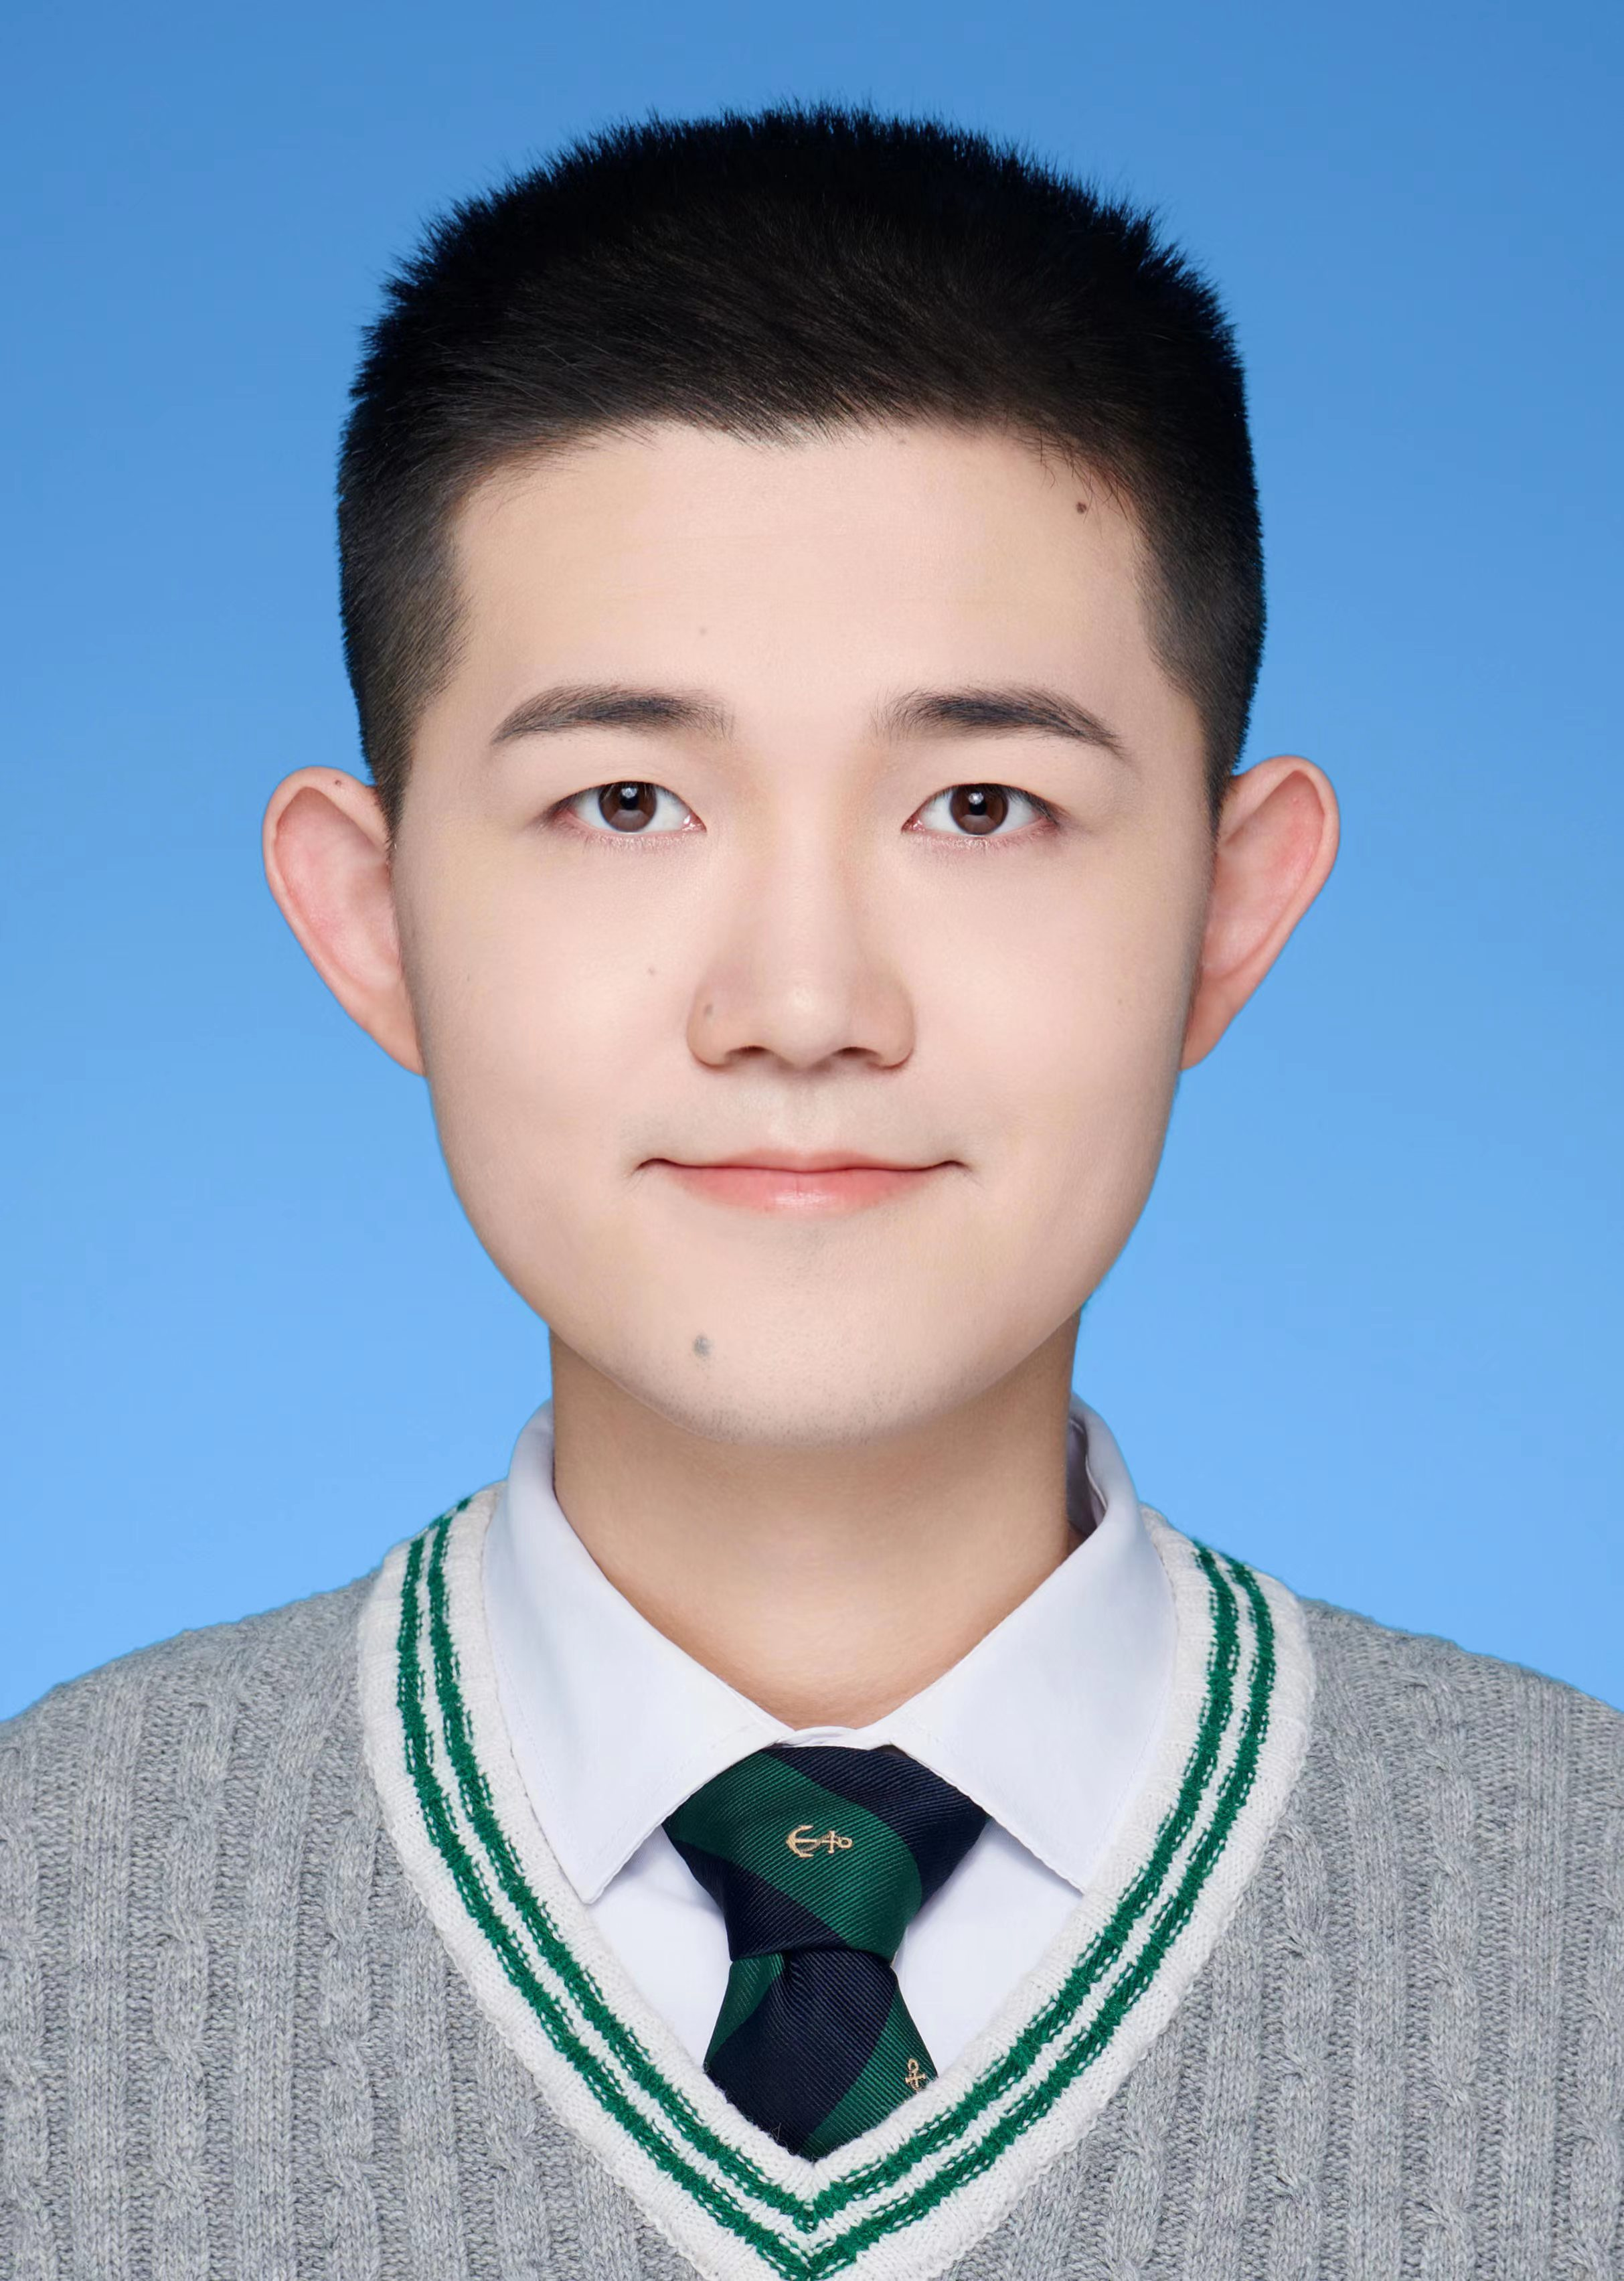
\includegraphics[width=0.88in]{avatar-college}} & \scshape{阮彦涵} & \pbar{React}{0.8} \\
    & \email{ruanyanhan@whu.edu.cn} & \pbar{ES6}{0.8} \\
    & \phone{(+86) 173-1836-1969} & \pbar{WebGIS}{0.5} \\
    & \linkedin[yo yo]{https://www.linkedin.com/in/yo-yo-974516289/} & \pbar{Express}{0.6} \\
    & \github[gitee.com/yohoyh]{https://gitee.com/yohoyh} & \pbar{Jquery}{0.6}
  \end{tabu}
}

\section{\faGraduationCap\ 教育背景}
\datedsubsection{\textbf{武汉大学 (WHU)}, 武汉, 中国}{2022 -- 至今}
\textit{在读硕士研究生} \  土木水利工程,预计 2024 年 7 月 毕业
\datedsubsection{\textbf{西北农林科技大学 (NWAFU)}, 陕西, 中国}{2018 -- 2022}
\textit{学士学位} \ 水利水电工程 
% \textit{B.S.} in Water Resources and Hydropower Engineering

\section{\faUsers\ 项目经历}
% 横沙项目
\datedsubsection{\textbf{碳中和大数据平台} \ 上海, 中国}{2023 年 5 月 -- 至今}
\role{与地方政府部门合作}{React | Antd | Express | ECharts | Resium}
% Brief introduction: The platform aims to enable carbon-neutral assessment and agricultural land information management on the islands.The main technical highlights are as follows:
\begin{itemize}
  \item 借助ES6+现代语法提升开发效率和代码可读性:通过运用最新的JavaScript语法,并提升代码的开发效率、可读性和可维护性
  \item 对可重复使用的实用函数进行封装:通过实现针对Cesium重新渲染事件的节流以及点击事件的防抖等功能,有效提高代码的可维护性和复用性
  \item 通过使用相对单位实现灵活的屏幕适配:采用相对单位作为屏幕适配的基准,使得项目能够自适应不同设备和屏幕尺寸的需求和变化
  \item 利用高阶组件(HOC)进行登录验证:结合React中的状态提升,将登录验证的高阶组件包裹到需要控制的组件中,提供更高层次的复用扩展性
  \item 引入懒加载提升性能和用户体验:借助钩子函数和节流的技术手段,通过在指定的高度范围内优化实体加载,可以显著提高项目的性能和用户体验
\end{itemize}

% 清美+宁夏
\datedsubsection{\textbf{数字水稻平台} \ 武汉, 中国}{2022 年 3 月 -- 2022 年 11 月}
\role{基于国家级重点项目}{Jquery | Express | ECharts | OpenLayers}
% Brief introduction: The platform aims to enable carbon-neutral assessment and agricultural land information management on the islands.The main technical highlights are as follows:
\begin{itemize}
  \item 区域田块智能管理,功能丰富,详细的开发文档编写,有效的管理和开发
  \item 系统全栈进行严格的安全验证,并具有较好的安全防范措施
  \item 采用双指针算法,将时间复杂度从 \(\mathbf{\mathit{o(n^{2})}}\) 降低到 \(\mathbf{\mathit{o(n)}}\),并对遥感图像进行预处理,提高加载150\%速度
  % \item Utilize dual-pointer algorithm to reduce time complexity from \(\mathbf{\mathit{o(n^{2})}}\) to \(\mathbf{\mathit{o(n)}}\), and preprocess remote sensing images for 150\% speed increase.
\end{itemize}

% Reference Test
%\datedsubsection{\textbf{Paper Title\cite{zaharia2012resilient}}}{May. 2015}
%An xxx optimized for xxx\cite{verma2015large}
%\begin{itemize}
%  \item main contribution
%\end{itemize}

% \section{\faCogs\ Skills}
% \begin{itemize}[parsep=0.5ex]
%   \item Programming Languages: C == Python > C++ > Java
%   \item Platform: Linux
%   \item Development: Web, xxx
% \end{itemize}

% \section{\faHeartO\ Honors and Awards}
% \datedline{\textit{\nth{1} Prize}, Award on xxx }{Jun. 2013}
% \datedline{Other awards}{2015}

\section{\faCalendarCheckO\ 获奖情况}
\begin{itemize}[parsep=0.5ex]
  \item 2022浙江大学计算机程序设计能力考试 (95 分/100 分)
  \item 2022 ACM-ICPC 优胜奖  \hspace{6em}  • 2020全国大学生数学竞赛 二等奖
  \item 2020美国大学生数学建模竞赛 三等奖  \hspace{6em} • 2021软件著作 两项

\end{itemize}

\section{\faPlusCircle\ 其他}
\begin{itemize}[parsep=0.5ex]
  \item 英语六级:539分,日常会话,熟练阅读英文文档
\end{itemize}

%% Reference
%\newpage
%\bibliographystyle{IEEETran}
%\bibliography{mycite}
\end{document}
